% !TeX program = lualatex

% Author: Malte, DE7LMS
% Year: 2022
% TH203 capacitor with label m33


\usepackage{siunitx}

\usepackage{amsmath}
\usepackage{unicode-math}
\setmathfont{Fira Math}
\setmathfont[range=up]{Roboto}
\setmathfont[range=it]{Roboto-Italic}
\setmathfont[range=\int]{Fira Math}
\usepackage[euler]{textgreek}

\begin{document}

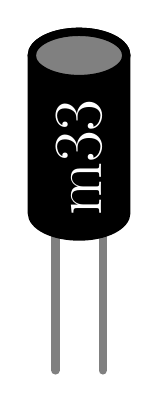
\begin{tikzpicture}
  \draw[line width=3pt, gray, line cap=round]
    (-.3,-1) -- ++(0,-3)
    (.3,-1) -- ++(0,-3);
  \filldraw[line width=3pt]
    (.6,-2)
    arc[start angle=0, end angle=-180, x radius=6mm, y radius=3mm]
    -- (-.6,0)
    arc[start angle=180, end angle=0, x radius=6mm, y radius=3mm]
    -- cycle;
  \filldraw[fill=gray,line width=3pt] (0,0) circle[x radius=6mm, y radius=3mm];
  \node[rotate=90, white, font=\Huge] at (0,-1.3) {m33};
\end{tikzpicture}

\end{document}


